\documentclass{scrartcl}
\usepackage[a4paper,left=1in,right=1in,top=1.2in,bottom=1in]{geometry}
\usepackage{siunitx}
\usepackage{graphicx}
\usepackage{mathtools}
\setkomafont{disposition}{\normalfont\bfseries}
\newcommand*\diff{\mathop{}\!\mathrm{d}}
\newcommand*\Diff[1]{\mathop{}\!\mathrm{d^#1}}
\newcommand*\colvec[3][]{
    \begin{pmatrix}\ifx\relax#1\relax\else#1\\\fi#2\\#3\end{pmatrix}
}

%title
\title{Exercise 08:\\Principal Component Analysis}
\subtitle{Theoretical Neuroscience II}
\author{Johannes G\"atjen \and Lorena Morton}

%use these for structure/overview
\newcommand\Question{%
  \textbf{Question:}%
}
\newcommand\Answer{%
  \textbf{Answer:}%
}
\renewcommand{\arraystretch}{1.2}


\begin{document}
\maketitle


\begin{figure}[h]
\centering
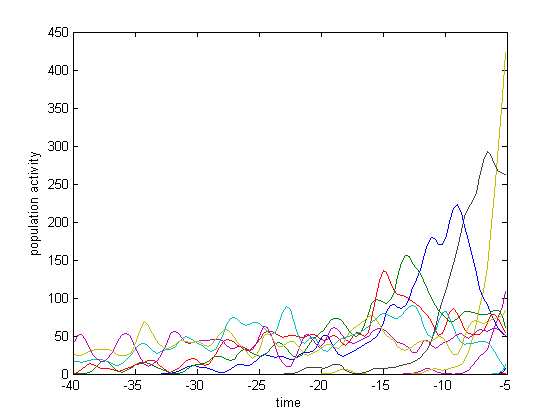
\includegraphics[trim = {0.7cm 0.3cm 1cm 0.7cm}, width=0.75\textwidth, clip]{../pics/orig_time}
\caption{Activity of all populations over time, averaged over all recordings.}
\label{}
\end{figure}

\begin{figure}[h]
\centering
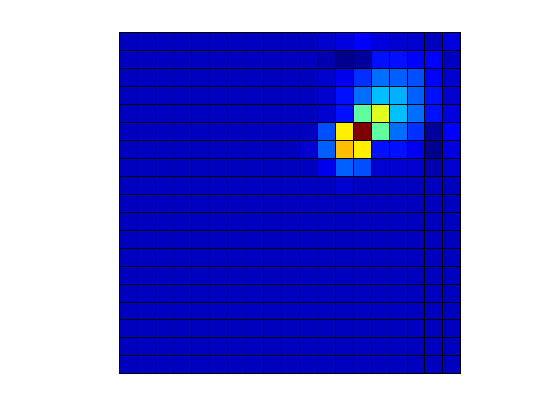
\includegraphics[trim = {1.7cm 0.5cm 1cm 1.7cm}, width=0.75\textwidth, clip]{../pics/orig_cov}
\caption{Covariance matrix of neuron populations.}
\label{}
\end{figure}

\begin{figure}[h]
\centering
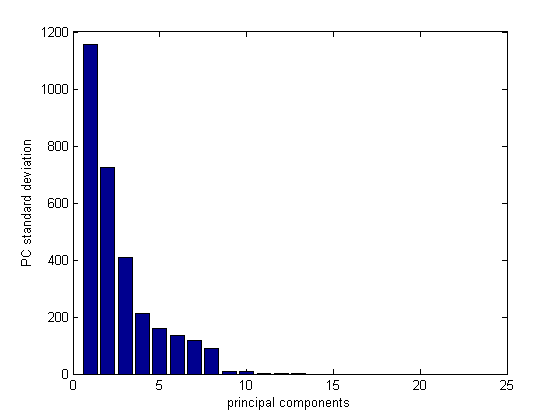
\includegraphics[trim = {0.55cm 0.3cm 1cm 0.7cm}, width=0.75\textwidth, clip]{../pics/pc_magn}
\caption{Standard deviation of the principal components. Three principal components have a medium to high standard deviation. Five further components have a low standard deviation and the remaining components have almost zero variance.}
\label{}
\end{figure}

\begin{figure}[h]
\centering
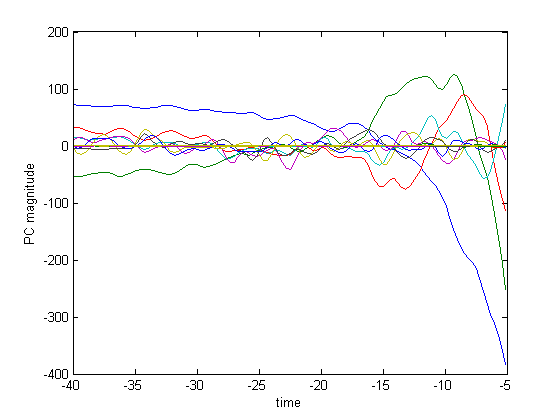
\includegraphics[trim = {0.6cm 0.3cm 1cm 0.7cm}, width=0.75\textwidth, clip]{../pics/pc_time}
\caption{Magnitude of principal components over time.}
\label{}
\end{figure}

\begin{figure}[h]
\centering
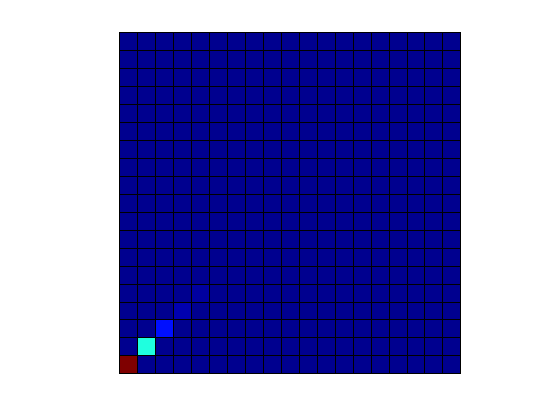
\includegraphics[trim = {1.7cm 0.5cm 1cm 1.7cm}, width=0.75\textwidth, clip]{../pics/pc_cov}
\caption{Covariance matrix of the principal components. As expected, only the diagonal elements are non-zero.}
\label{}
\end{figure}

\begin{figure}[h]
\centering
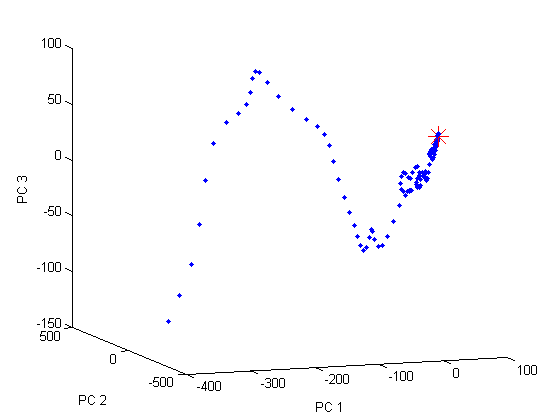
\includegraphics[trim = {0.4cm 0.1cm 1cm 0.7cm}, width=0.75\textwidth, clip]{../pics/trace_avg}
\caption{Trajectory through the space of the first three principal components, averaged over all recordings. The red star indicates the start state.}
\label{}
\end{figure}

\begin{figure}[h]
\centering
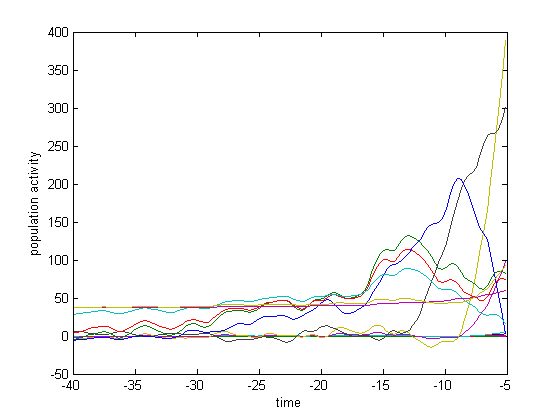
\includegraphics[trim = {0.7cm 0.3cm 1cm 0.7cm}, width=0.75\textwidth, clip]{../pics/denoised}
\caption{The first three principal components projected back into the original space, averaged over all recordings. We can see that a burst is typically preceded by moderate synchronous activity of three populations, sequentially followed by increasingly higher activity of three further populations.}
\label{}
\end{figure}

\begin{figure}[h]
\centering
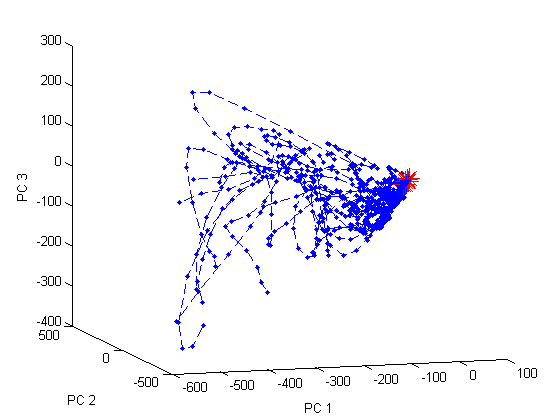
\includegraphics[trim = {0.4cm 0.1cm 1cm 0.7cm}, width=0.75\textwidth, clip]{../pics/traces_all}
\caption{Trajectory through the space of the first three principal components for all recordings. The red stars indicate the start state.}
\label{}
\end{figure}


\end{document}